\documentclass[12pt]{article}

% Include extracted results from CSV files
% LaTeX commands for inline results
% Auto-generated — do not edit manually

\newcommand{\bestModelName}{GPT-5}
\newcommand{\bestMeanMicroF}{0.6667}
\newcommand{\bestMeanMacroF}{0.5996}
\newcommand{\bestMeanWeightedF}{0.6597}

\newcommand{\testSetSize}{1549}
\newcommand{\trainingSetSize}{38,451}
\newcommand{\numModels}{5}
\newcommand{\numTasks}{4}

\newcommand{\friedmanChiSquare}{39.57}
\newcommand{\friedmanP}{< 0.0001}
\newcommand{\kendallW}{0.275}
\newcommand{\kruskalH}{25.71}
\newcommand{\kruskalP}{< 0.0001}
\newcommand{\etaSquared}{0.117}

\newcommand{\bestThemesModel}{GPT-OSS}
\newcommand{\bestThemesMicroF}{0.6300}
\newcommand{\bestSentimentModel}{GPT-5}
\newcommand{\bestSentimentMicroF}{0.7411}
\newcommand{\bestPoliticalpartiesModel}{GPT-5}
\newcommand{\bestPoliticalpartiesMicroF}{0.9031}
\newcommand{\bestSpecificthemesModel}{GPT-5}
\newcommand{\bestSpecificthemesMicroF}{0.4750}

% Essential packages
\usepackage[utf8]{inputenc}
\usepackage[T1]{fontenc}
\usepackage[english]{babel}
\usepackage{geometry}
\geometry{margin=2.5cm}
\usepackage{booktabs}
\usepackage{longtable}
\usepackage{ltcaption}
\usepackage{multirow}
\usepackage{array}
\usepackage{tabularx}
\usepackage{colortbl}
\usepackage{graphicx}
\usepackage{xcolor}
\usepackage{tikz}
\usepackage{authblk}
\usepackage{pdflscape}
\usepackage{afterpage}
\usepackage{amsmath}
\usepackage{algorithm}
\usepackage{algorithmic}
\usepackage{float}

% Bibliography
\usepackage[backend=biber,style=authoryear,sorting=nyt]{biblatex}
\addbibresource{../bibliography/library.bib}
\addbibresource{../bibliography/LLM_tool.bib}

% Hyperref setup
\usepackage[unicode=true,colorlinks=true,linkcolor=blue,citecolor=blue,urlcolor=blue]{hyperref}
\usepackage{cleveref}

% Configure cleveref
\crefname{table}{Table}{Tables}
\Crefname{table}{Table}{Tables}
\crefname{figure}{Figure}{Figures}
\Crefname{figure}{Figure}{Figures}

% TikZ libraries
\usetikzlibrary{positioning,backgrounds,fit,shapes,shapes.geometric,calc,matrix,arrows.meta,patterns}
\usepackage{pgfplots}
\pgfplotsset{compat=1.17}
\usepackage{csquotes}

% Define colors for the pipeline
\definecolor{llmcolor}{RGB}{59, 130, 246}
\definecolor{bertcolor}{RGB}{34, 197, 94}
\definecolor{evalcolor}{RGB}{239, 68, 68}
\definecolor{datacolor}{RGB}{251, 146, 60}

\title{\textbf{LLM Tool: A Hybrid Pipeline for Automated Large-Scale Text Annotation Using Local Language Models and BERT Classifiers}}

\author[1]{Antoine Lemor}
\author[2]{Shannon Dinan}
\author[3]{Jérémy Gilbert}
\affil[1]{Université de Montréal}
\affil[2]{Université Laval}
\affil[3]{Western University}

\date{}

\begin{document}

\maketitle
\thispagestyle{empty}

\begin{abstract}
\noindent
As access to local large language models (LLM) has expanded, so too has their use by social scientists. This innovation has rapidly led to legitimate debates regarding the ethical use of artificial intelligence in social science research, and questions about how to ensure accessibility and transparency. This article presents LLM Tool, a hybrid data processing workflow that combines LLMs with transformer classifiers for automated and scalable text annotation. The system includes an end-to-end pipeline for processing, training, evaluation, and deployment. This workflow democratizes large-scale text annotation for computational social science while also providing a means to ensure the transparent and valid use of these methods.

Empirical validation on 1,593 Canadian political texts shows models trained on LLM annotations achieve 66.73\% Micro F1, outperforming the human-trained models (46.01\% Micro F1) by 45\%. This advantage stems from systematic machine consistency versus human variability. The quality of the workflow is verified using three dataset configurations to  validate scalability and performance.
\end{abstract}

\noindent\textbf{Keywords:} large language models, text annotation, computational social science, transformer classifiers, methodological transparency.

\vspace{0.4cm}

\noindent\textbf{Funding:} This research was made possible by a \textit{Programme d’appui à l’innovation pédagogique} grant from the Faculté des Sciences Sociales of Université Laval. 
\newpage

\section{Introduction}

The growing accessibility of large language models (LLMs) has prompted a rapid expansion of their use in social science, as researchers turn to these models to analyze increasingly large textual datasets generated by the big data era. Many projects now rely on zero- or few-shot applications of LLMs for text classification, summarization, and annotation. Yet, these approaches raise long-standing methodological and ethical concerns by challenging the core principles of validity, reproducibility, and research transparency. The use of these models also carries significant environmental costs. The question, then, is not how to restrict the use of artificial intelligence in social research, but how to ensure that its application remains accessible, transparent, and methodologically sound, augmenting the work of social scientists rather than replacing it \parencite{grimmer_stewart13, do_etal24}.

This article introduces a hybrid data processing workflow, LLM tool, that combines local LLMs with transformer classifiers for automated and scalable text annotation. The system includes an end-to-end pipeline for processing, training, evaluation, and deployment. By operationalizing these models in a controlled and local workflow, the LLM tool democratizes large-scale text annotation for computational social science while also supporting methodological transparency and reproducibility.

LLM Tool can process multiple data formats (CSV, Excel, Parquet, RData, PostgreSQL) through structured prompts with dynamic JSON validation. It integrates open-source LLMs (including Gemma, Llama, Nemotron, DeepSeek-R1, GPT-OSS) via Ollama and provides over 30 transformer models including DeBERTa-v3, RoBERTa, ELECTRA, as well as multilingual variants. Automatic model selection optimizes architectures based on language and task complexity. Training transformer classifiers through LLM-processed data improves efficiency by 100-1000x: while LLMs take between 27-112 seconds per document, BERT models complete the task in under one second. The tool operates entirely locally, ensuring data privacy without API dependencies. 

Empirical validation on 1,593 Canadian political texts shows models trained on LLM annotations achieve 66.73\% Micro F1, outperforming the human-trained models (46.01\% Micro F1) by 45\%. This advantage stems from systematic machine consistency versus human variability. Workflow is quality is further verified using three dataset configurations -- Small (1,343 sentences), Large (5,753 sentences), and Extra-Large (12,000 sentences with isolated test data) -- demonstrating both scalability and performance. 

\section{The Promise and Limitations of Large Language Models in Social Sciences}

Large language models have inspired considerable optimism among computational social scientists for their apparent ability to offer a solution to one of the field’s most persistent challenges: large-scale text annotation. The production of labeled data has typically required extensive human effort, clear coding guidelines, and costly quality control. LLMs, in contrast, appear to provide an efficient solution because they draw on vast pre-trained knowledge to perform complex classification and extraction tasks with minimal supervision. This prospect of rapid scaling has made them attractive for research programs that would otherwise demand prohibitive amounts of time and human resources.

Evidence, nevertheless, tempers this promise. While LLMs can achieve high accuracy on straightforward and unambiguous labeling tasks such as binary political affiliation detection, sometimes even outperforming supervised models and human annotators \parencite{tornberg24a, gilardi_etal23}, they perform far less reliably on the complex and multidimensional coding schemes common in social science research \parencite{halterman_keith25, alizadeh_etal24a}. Open-source models, in particular, show a limited capacity to follow detailed codebooks, even when these provide explicit definitions and examples \parencite{halterman_keith25}. 

\subsection{Performance Limits and Structural Constraints}

The performance gap between proprietary models like GPT-4 and open alternatives remains substantial on political text classification benchmarks \parencite{alizadeh_etal24a}, and even the most advanced systems struggle when annotation requires sustained attention to nuanced and context-dependent distinctions. Ultimately, it appears that task complexity, rather than model architecture or raw capacity, determines whether LLMs fulfill their promise or reveal their current limits.

A second set of concerns involves the conditions under which many LLMs are available to researchers. Commercial API-based models operate as black boxes, limiting validity checks and reproducibility. For instance, researchers using zero-shot applications in which the model is tasked directly with annotating a dataset without a specific training task may obtain unpredictable results. Moreover, because these API-based systems are continuously updated or replaced, results obtained at one point in time may not be replicable later. In addition to these validity and reproducibility concerns, model hallucinations undermine research credibility for high-quality annotations \parencite{rateria_singh24}. The mechanisms behind proprietary models remain opaque, which limits error analysis and auditing in downstream applications \parencite{zhao_etal24}. Pricing that scales with data volume and model complexity also creates barriers for unfunded teams and for institutions outside well-resourced settings. At the scale of millions of sentences, end-to-end annotation with decoder LLMs becomes practically infeasible: local models would require months or years of computing for inference alone, whereas commercial endpoints imply costs that exceed typical research budgets. 

As API versions change, models are deprecated, and access conditions shift, reproducibility is further compromised, and past analyses may become impossible to replicate \parencite{weber_reichardt23}. Off-the-shelf multilingual models also show uneven performance across languages and domains, with weaker results in low-resource contexts \parencite{bhat_varma23, mets_etal24}. Data privacy concerns restrict the use of external services when corpora contain sensitive material. Political and demographic biases in training data raise important ethical issues for social and political categorization \parencite{mcgee23, rozado23, dong_etal23}. These constraints underscore the need for transparent, auditable, and locally executable alternatives that support equity as well as scientific reliability.

\subsection{Fine-Tuned LLMs: Improvements, Data Needs, and Trade-Offs}

An alternative to zero-shot LLMs is the use of fine-tuned models. Fine-tuning involves training a decoder-based language model on a specific task using labeled examples, allowing the model to adapt its general language understanding to the particular annotation requirements of a research project. These models show clear improvements in complex text annotation tasks, addressing many of the limitations observed in zero-shot approaches \parencite{alizadeh_etal24a, halterman_keith25}. For political text classification, fine-tuned models also outperform few-shot prompting strategies when provided with even modest amounts of training data \parencite{alizadeh_etal24a, wang_etal24}, though the optimal choice between fine-tuning and prompting depends on task complexity and dataset size \parencite{chen_etal23}.

However, the fine-tuning process still requires labeled data. While fine-tuning may require fewer examples than training classical supervised models from scratch, researchers must still invest time and resources in creating training datasets. For low-resource scenarios, fine-tuned models may match traditional approaches only when training sets reach several hundred or thousand examples \parencite{wang_etal24}. Fine-tuning therefore shifts rather than solves the fundamental challenge. Instead of annotating entire corpora, researchers must now annotate training sets of sufficient size and quality to produce reliable models.

\section{Transfer Learning and BERT-Family Models}

An alternative to zero-shot LLMs is to train task-specific transformer models, such as those in the BERT family. This form of transfer learning leverages the knowledge acquired during large-scale pre-training to improve performance on specialized annotation tasks,  adapting general language understanding to new tasks with relatively small amounts of labeled data while requiring far fewer labeled examples than if the model were trained from scratch. This is a practical compromise between zero-shot approaches, which rely entirely on a model’s pre-existing knowledge, and classical supervised methods, which are trained from scratch on task-specific data. This approach has demonstrated substantial reductions in labeled data requirements: pre-trained models achieve strong performance with far fewer examples\parencite{laurer_etal23, wankmuller24}.

The efficiency gains from transfer learning prove to be substantial across diverse political science applications. Pre-trained BERT models can match the performance of classical supervised models while requiring only a fraction of the training data. For example, 500 labeled texts suffice where traditional approaches need 5,000, with improvements of 10 to 18 percentage points over non-transfer methods \parencite{laurer_etal23}. These gains translate well to imbalanced datasets where certain categories may be rare. Transfer learning models outperform conventional machine learning approaches across variations in text style, domain, and training set size, demonstrating robustness beyond specific tasks or corpora \parencite{wankmuller24}. Domain-specific applications confirm the practical value of this approach, from classifying and measuring political concepts to extracting sentiment \parencite{dreier_etal25, matsuo_fukumoto25, bonikowskiPoliticsUsualMeasuring2022}.


\subsection{Training Data Quality}

Transfer learning's efficiency depends on the quality of the supervision it receives during fine-tuning. Traditional approaches rely on human annotation. Yet annotators show variable consistency even on well-defined tasks. Furthermore, inter-annotator agreement scores frequently fall in the moderate range for complex political text annotation. Annotation fatigue explains some of these issues. As annotators process thousands of texts, attention diminishes and error rates increase, with expert annotators missing identifiable instances  due to the cognitive demands of sustained coding \parencite{do_etal24}. Training costs and time requirements remain important even when target sample sizes drop, and quality control becomes increasingly difficult when annotation is distributed across multiple coders.

Alternative approaches to generating training data remain limited. Rule-based systems, such as dictionaries, can produce labels at scale but require extensive domain expertise to construct and struggle with the context-dependent cases typical of social science text. Weak supervision from naturally occurring labels can address specific tasks but cannot be generalized across the diverse annotation challenges researchers face \parencite{matsuo_fukumoto25}. A tension therefore persists: transfer learning models require training data that are both large and consistent, yet available methods for generating such data either require considerable human effort or apply only to narrow task structures. A hybrid approach offers the solution, using LLMs not as direct classifiers but as generators of labeled data to efficiently train transformer-based models for  downstream tasks.

\section{Hybrid Architectures}

Hybrid architectures represent a new generation of computational annotation frameworks that combine the interpretive capacity of decoder-based LLMs with the efficiency, consistency, and scalability of encoder-based LLMs. We contend they offer a promising approach to social science text annotation. A model in which human expertise, LLM-based interpretation, and algorithmic inference are not opposed but articulated within a single, recursive workflow. 

The underlying principle is straightforward (see Figure \ref{fig:hybrid_architecture}): the LLM produces contextual annotations, humans audit and correct its outputs, and a transformer model is trained from these refined labels to apply them consistently at scale. The result is a system that merges the flexibility of decoder-based LLMs with the scalability of encoder-based ones.

Hybrid approaches have explored various forms of collaboration between human expertise and machine learning. Some frameworks rely on multi-stage designs in which LLMs generate preliminary labels, automated filters estimate confidence, and human coders adjudicate ambiguous cases \parencite{wang_etal24a}. Others combine model predictions with targeted human correction to strengthen conceptual coherence \parencite{dreier_etal25}. In several cases, transformer classifiers trained on LLM-generated data achieve performance close to that of models trained on human annotations, suggesting that LLMs can function as scalable annotation sources for downstream supervised models \parencite{heseltineLargeLanguageModels2024, pangakisKnowledgeDistillationAutomated2024}. 

\begin{figure}[t!]
\centering
\resizebox{\textwidth}{!}{%
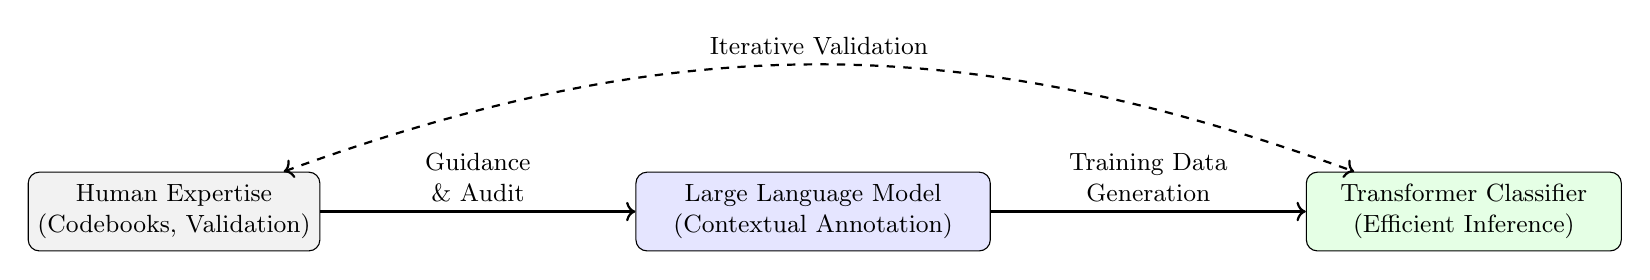
\begin{tikzpicture}[node distance=4cm, every node/.style={align=center, font=\small}]
    \node (human) [draw, rounded corners, fill=gray!10, minimum width=3.5cm, minimum height=1cm] {Human Expertise\\(Codebooks, Validation)};
    \node (llm)   [draw, rounded corners, fill=blue!10, minimum width=4.5cm, minimum height=1cm, right=of human] {Large Language Model\\(Contextual Annotation)};
    \node (bert)  [draw, rounded corners, fill=green!10, minimum width=4.0cm, minimum height=1cm, right=of llm] {Transformer Classifier\\(Efficient Inference)};

    \draw[->, thick] (human) -- node[above]{Guidance\\ \& Audit} (llm);
    \draw[->, thick] (llm) -- node[above]{Training Data\\Generation} (bert);
    \draw[<->, thick, dashed] (human) to[bend left=20] node[above, sloped]{Iterative Validation} (bert);
\end{tikzpicture}%
}
\caption{Conceptual structure of a hybrid annotation architecture integrating human, LLM, and transformer components.}
\label{fig:hybrid_architecture}
\end{figure}

\subsection{Empirical Advances and Persistent Fragmentation}

Despite these advances, existing hybrid systems remain fragmented. They generally rely on proprietary APIs, target narrow tasks or domains, and rarely provide reproducible infrastructures that other researchers can reuse. As several systematic reviews have underlined, reproducibility represents a persistent weakness in computational annotation. Even published methods that appear well-documented often fail to reproduce because of undocumented preprocessing steps, missing code, or unstable model versions \parencite{chen_etal23, weber_reichardt23}. The opacity of LLM mechanisms further complicates validation, as researchers have limited insight into why models produce particular outputs or when they fail \parencite{zhao_etal24}. 

For commercial APIs, replication becomes nearly impossible once endpoints change or models are deprecated. These structural issues converge with the broader problem of validation inconsistency identified in the literature. Automated text analysis studies differ widely in their evaluation practices, often reporting predictive accuracy without verifying whether models capture the intended constructs or generalize beyond their training contexts \parencite{park_montgomery25, bernhard-harrer_etal25, glockner_etal20}. As \textcite{tornberg24b} and \textcite{atreja_etal24} have noted, this combination of opacity and instability has created what resembles a methodological “Wild West,” where prompt design and implementation details can decisively influence results.

\subsection{Toward Open, Reproducible, and Accessible Pipelines}

Thus, three methodological gaps continue to limit cumulative progress. First, few systematic comparisons exist between LLM-generated and human-generated training data under controlled conditions using isolated test sets \parencite{park_montgomery25, bernhard-harrer_etal25}. Second, hybrid workflows remain project-specific, combining heterogeneous tools and scripts in ways that undermine reproducibility and prevent cumulative validation \parencite{chen_etal23, weber_reichardt23}. Third, the field lacks an integrated open-source framework capable of deploying a complete hybrid architecture locally while ensuring full reproducibility, transparency, and accessibility. 

To the authors’ knowledge, no existing system combines local LLM-based annotation, transformer fine-tuning, and large-scale inference within a single pipeline that automatically documents every parameter and environment configuration for verifiable replication. Nor does any framework provide an accessible command-line interface that allows researchers to execute the entire process without programming expertise. The absence of such an infrastructure limits the democratization of hybrid methods and concentrates computational capacity within well-resourced institutions. The promise of hybrid architectures remains clear, yet realizing it requires open, systematic, and locally executable pipelines that align scientific rigor with equitable access.

\section{The LLM Tool Concept}

\subsection{Hybrid Foundation}

LLM Tool was developed to address the methodological and infrastructural limitations identified above. It provides the first open-source implementation of a fully local hybrid pipeline that unites decoder-based and encoder-based language models in a single reproducible workflow. The system enables any researcher to perform large-scale text annotation without reliance on commercial APIs (even though the package includes API functionalities) or advanced programming skills. It integrates transparency, accessibility, and empirical validation into a unified framework.

The pipeline combines two complementary components. Decoder-based LLMs interpret annotation guidelines and produce structured contextual labels, while transformer-based models generalize these annotations across entire corpora. Local execution through open-source LLMs removes dependency on external services and ensures the confidentiality of sensitive data. This configuration also eliminates recurring API costs that make large-scale annotation prohibitively expensive for most institutions. Once the LLM has produced an annotated dataset, the pipeline trains encoder-based models such as BERT and its derivatives to reproduce the labeling logic with far greater efficiency. This division of tasks allows the system to handle corpora of millions of sentences within hours instead of months, a scale impossible to reach through direct LLM inference alone.

The workflow operates entirely on local machines and can be executed through a command-line interface without needing any coding. This feature ensures that researchers without programming expertise can process, train, and evaluate models in a reproducible way. Each stage of the workflow is automatically documented, including model parameters, prompts, software versions, and environment settings, which guarantees full traceability and replicability.

The package integrates extensive technical infrastructure to support diverse research contexts. It provides several LLM provider architectures with fully local execution options as well as commercial API if needed, over 50 transformer models with automatic selection capabilities, comprehensive data characterization across 75+ languages, integrated quality assurance through multiple validation mechanisms, and three command-line interface modes for annotation, training, and validation workflows. The benchmarking architecture enables systematic model comparison through standardized protocols addressing methodological gaps in existing comparative studies. Complete technical specifications, model architectures, and implementation details are documented in Appendix~\ref{sec:technical-infrastructure}.

\subsection{Pipeline Architecture}

\begin{figure}[b!]
\centering
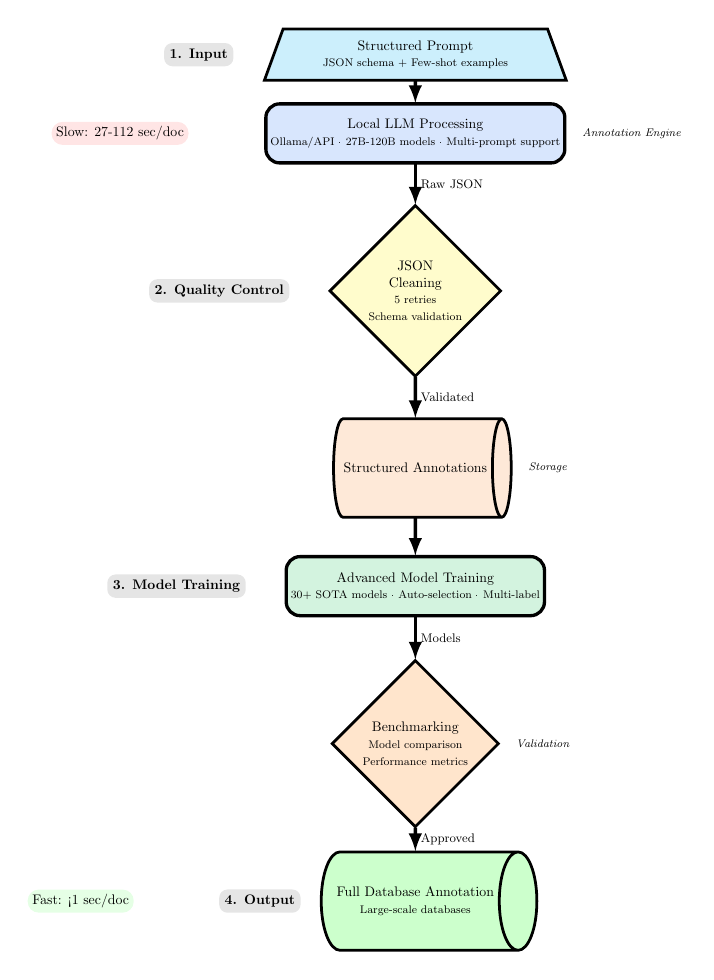
\begin{tikzpicture}[scale=0.5, transform shape,
    node distance=2cm,
    box/.style={rectangle, draw=black, line width=1pt, minimum width=4cm, minimum height=1cm, align=center, rounded corners=5pt, font=\normalsize},
    process/.style={rectangle, draw=black, line width=1.2pt, minimum width=5cm, minimum height=1.5cm, align=center, rounded corners=5pt, font=\normalsize},
    data/.style={cylinder, draw=black, line width=1pt, shape border rotate=0, minimum width=2 .5cm, minimum height=1cm, align=center, font=\normalsize},
    prompt/.style={trapezium, trapezium angle=70, draw=black, line width=1pt, minimum width=4.5cm, minimum height=1.3cm, align=center, font=\normalsize},
    verify/.style={diamond, draw=black, line width=1pt, minimum width=3.5cm, minimum height=3.5cm, align=center, font=\normalsize},
    arrow/.style={->, line width=1.2pt, >=latex},
    title/.style={font=\Large\bfseries},
    label/.style={font=\footnotesize\itshape, right=0.3cm},
    phase/.style={font=\normalsize\bfseries, fill=gray!20, rounded corners=3pt, inner sep=4pt}
]

% Step 1: Structured Prompt
\node[prompt, fill=cyan!20] (prompt) at (0, 11.5) {Structured Prompt\\{\footnotesize JSON schema + Few-shot examples}};
\node[phase, left=1cm of prompt] {1. Input};

% Step 2: LLM Processing
\node[process, fill=llmcolor!20] (llm) at (0, 9.5) {Local LLM Processing\\{\footnotesize Ollama/API · 27B-120B models · Multi-prompt support}};
\node[label] at (llm.east) {Annotation Engine};

% Step 3: JSON Validation & Cleaning
\node[verify, fill=yellow!20] (clean) at (0, 5.5) {JSON\\Cleaning\\{\footnotesize 5 retries}\\{\footnotesize Schema validation}};
\node[phase, left=1cm of clean] {2. Quality Control};

% Step 4: Structured Annotations
\node[data, fill=datacolor!20] (annotations) at (0, 1) {Structured Annotations};
\node[label] at (annotations.east) {Storage};

% Step 5: Advanced Model Training
\node[process, fill=bertcolor!20] (training) at (0, -2) {Advanced Model Training\\{\footnotesize 30+ SOTA models · Auto-selection · Multi-label}};
\node[phase, left=1cm of training] {3. Model Training};

% Step 6: Benchmarking & Verification
\node[verify, fill=orange!20] (verify) at (0, -6) {Benchmarking\\{\footnotesize Model comparison}\\{\footnotesize Performance metrics}};
\node[label] at (verify.east) {Validation};

% Step 7: Full Database Annotation
\node[data, fill=green!20] (database) at (0, -10) {Full Database Annotation\\{\footnotesize Large-scale databases}};
\node[phase, left=0.5cm of database] {4. Output};

% Arrows with labels
\draw[arrow] (prompt) -- (llm);
\draw[arrow] (llm) -- node[right, font=\small] {Raw JSON} (clean);
\draw[arrow] (clean) -- node[right, font=\small] {Validated} (annotations);
\draw[arrow] (annotations) -- (training);
\draw[arrow] (training) -- node[right, font=\small] {Models} (verify);
\draw[arrow] (verify) -- node[right, font=\small] {Approved} (database);


% Performance indicators
\node[fill=red!10, rounded corners] at (-7.5, 9.5) {Slow: 27-112 sec/doc};
\node[fill=green!10, rounded corners] at (-8.5, -10) {Fast: <1 sec/doc};

\end{tikzpicture}%
\caption{The LLM Tool pipeline: A comprehensive automated annotation system}
\label{fig:llm_tool_concept}
\end{figure}

The LLM Tool pipeline follows four main phases, from data input to large-scale annotation, as illustrated in Figure \ref{fig:llm_tool_concept}. The first phase, \emph{Input}, processes textual data from multiple formats including CSV, Excel, Parquet, RData, and PostgreSQL. It defines annotation tasks through structured prompts that include dynamic JSON schemas. Each prompt is validated automatically through on-the-fly Pydantic models, ensuring that LLM outputs conform to the expected structure. This approach allows researchers to customize annotation schemes and label hierarchies without modifying any code. 

The second phase, \emph{Quality Control}, verifies and cleans the raw LLM outputs. Each response is validated through successive checks, with up to five retries. The tool applies JSON repairs, regular expression cleaning, and schema validation to correct structural inconsistencies. All steps generate detailed logs, which include raw responses, cleaned versions, and validation outcomes. Incremental saving guarantees that no data is lost during long-running processes. These procedures make the annotation process transparent and reproducible, countering the reproducibility problems observed in existing studies \parencite{chen_etal23, weber_reichardt23, zhao_etal24}.

The third phase, \emph{Model Training}, converts LLM-generated annotations into efficient transformer classifiers. The system provides access to over 50 models across language-specific, state-of-the-art, and domain-specialized architectures. The model selector identifies the most appropriate architecture according to the detected language, task complexity, and computational resources. The training process includes stratified multi-label classification, balanced sampling for imbalanced datasets, and parallel GPU training to accelerate computation. Once trained, these classifiers can annotate millions of texts in seconds, while maintaining consistent labeling accuracy.

The final phase, \emph{Output}, deploys the trained model for large-scale annotation and evaluation. It performs full-corpus inference through distributed processing, producing outputs in multiple formats such as CSV with evaluation metrics, model checkpoints with metadata, and inference-ready files. Benchmarks and validation reports document model performance, ensuring that every result can be replicated. Figure \ref{fig:llm_tool_concept} summarizes the complete workflow and its main validation checkpoints.

By packaging these capabilities into a unified, locally executable tool, we democratize access to state-of-the-art text annotation methods while ensuring complete data privacy and eliminating dependency on external services. LLM Tool presents three core innovations in automated text annotation. First, it treats LLM annotations as training data that can outperform human labels due to their systematic consistency across large datasets. Second, the tool operates entirely through local processing with open-source models to ensure data privacy and eliminate external API dependencies. Third, the validation architecture implements multiple dataset configurations with complete test isolation to verify model performance.

The pipeline is designed for adaptability across domains and languages through modular components. Users can substitute and compare LLMs, modify prompt templates, or change model architectures through configuration files. Multiple data formats and annotation schemas are supported without the user having to make modifications to the underlying code. This design enables deployment across research contexts, including parliamentary transcripts, media articles, and policy documents.

\newpage
\section{Methods and Data}

\subsection{Data Collection and Corpus Composition}
To validate the hybrid pipeline, multiple analyses were conducted using a corpus of political and media data from Canada containing 20,000 individual sentences. This dataset combines parliamentary debates at the federal and provincial (Quebec) levels from the Agora+ dataset (CAPP, 2025a) with media coverage from thirteen anglophone and francophone front pages drawn from the Radar+ dataset (CAPP, 2025b).

A manually annotated sample of 1,593 sentences, produced by a team of five researchers, served to create a ground truth. Larger portions of the corpus are used for LLM training and validation. In all, there are three dataset configurations: Small (1,343 sentences), Large (5,753 sentences), and Extra-Large (12,000 sentences with isolated test data). As the corpus includes both English and French texts, multilingual classification capabilities are required.

The textual data are divers, with the parliamentary component comprising House of Commons debates, including legislative discussions, question periods, and members’ statements, which are characterized by formal political discourse and specialized vocabulary. The media component consists of Canadian news articles, exposing models to diverse communication styles. This variety allows the hybrid pipeline to be evaluated across multiple registers and contexts.

\input{../results/outputs/tables/corpus_statistics_extracted.tex}

The corpus statistics show characteristics affecting model performance. The distribution between parliamentary texts and headlines varies across dataset configurations. Larger datasets have a more balanced representation. The Extra-Large configuration isolates test data completely, preventing data leakage.

\subsection{Annotation Schema}

The annotation schema belongs to the Center for Public Policy Analysis and identifies four dimensions: policy themes, specific themes, political parties, and sentiment. This captures both substantive content and political dynamics.

Textual data is classified into one of 21 major public policy themes.\footnote{Available in Annex A} These align with the Comparative Agendas Project (CAP) policy categories, which is a validated international typology used by more than 27 countries and 38 affiliated institutions (Jones et al. 2023). Each theme includes definitions and coding instructions. In addition, specific themes were classified to capture Canadian policy areas of interest to the research team: welfare state provisions and early learning programs. 

The political party dimension covers nine Canadian federal and Quebec provincial parties. Care must be taken, as parties with the same or similar names across levels represent distinct ideological positions. The sentiment dimension distinguishes between positive, neutral, and negative framings.

\begin{table}[h!]
\centering
\caption{Annotation category distribution}
\label{tab:categories}
\begin{tabular}{lrc}
\toprule
\textbf{Dimension} & \textbf{Categories} & \textbf{Description} \\
\midrule
Policy Themes & 21 & health, environment, economy, etc. \\
Specific Themes & 2 & welfare state, childcare \\
Political Parties & 10 & LPC, CPC, BQ, NDP, CAQ, etc. \\
Sentiment & 3 & positive, neutral, negative \\
\midrule
\textbf{Total} & \textbf{36} & \\
\bottomrule
\end{tabular}
\end{table}


\subsection{Manual Annotation Process}

The ground truth dataset comes from five annotators with expertise in Canadian politics. The annotators were trained using the CAP code book and provided with Canadian-specific guidelines. The Doccano platform was used as an annotation interface, notably to ensure unbiased coding and to facilitate quality monitoring. The team began by coding 100 sentences. The research leader and an assistant then reviewed annotations and compared them to resolve conflicts. Subsequent coding then continued after practice sessions and calibration exercises. This lead to a dataset in which each text received annotations from all five annotators.

Agreement metrics show moderate to substantial consistency across annotators, with a Krippendorff’s alpha for chance-corrected multi-annotator agreement with missing data ranging of 0.63 and a Fleiss' Kappa for multi-rater agreement of 0.96.

Category-specific metrics highlight variation in annotation difficulty. Policy theme X achieves a higher agreement (alpha here) compared with Policy theme Y. It also shows differences according to the annotation task, with Policy themes achieving higher agreement than political party identification. Substantive content proves easier to categorize than political attribution. Lower alpha values compared to kappa scores reflect different metric sensitivities.

\input{../results/outputs/tables/agreement_extracted.tex}


% Second diagram: Validation Pipeline
\begin{figure}[H]
\hspace*{+1cm} % Shift the entire diagram to the left
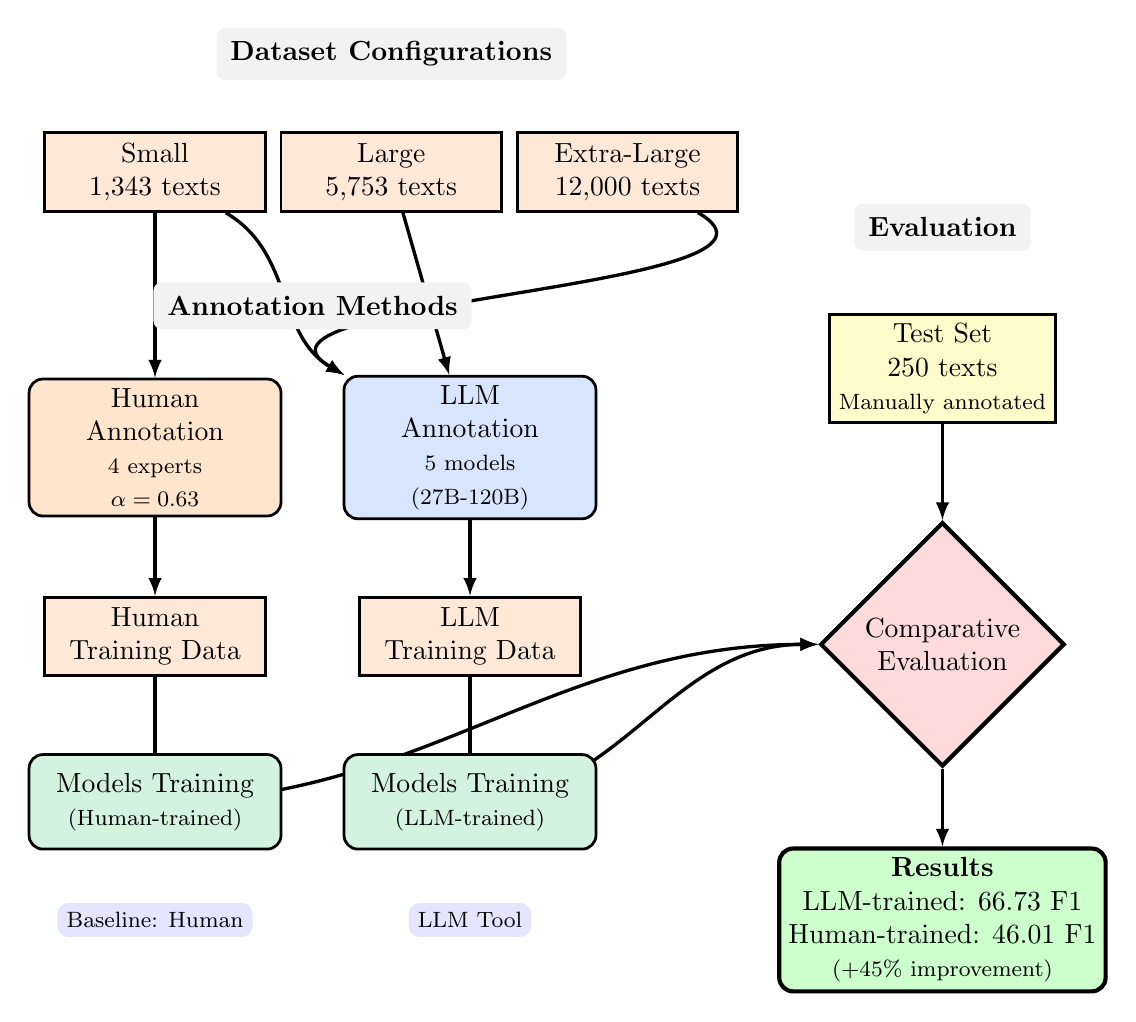
\begin{tikzpicture}[
    node distance=1.8cm,
    box/.style={rectangle, draw=black, line width=1pt, minimum width=2.2cm, minimum height=1.2cm, align=center, rounded corners=5pt, font=\normalsize},
    data/.style={rectangle, draw=black, line width=1pt, shape border rotate=90, minimum width=2.8cm, minimum height=1cm, align=center, font=\normalsize},
    human/.style={rectangle, draw=black, line width=1pt, minimum width=3.2cm, minimum height=1.2cm, align=center, rounded corners=5pt, font=\normalsize},
    llm/.style={rectangle, draw=black, line width=1pt, minimum width=3.2cm, minimum height=1.2cm, align=center, rounded corners=5pt, font=\normalsize},
    bert/.style={rectangle, draw=black, line width=1pt, minimum width=3.2cm, minimum height=1.2cm, align=center, rounded corners=5pt, font=\normalsize},
    eval/.style={diamond, draw=black, line width=1.5pt, minimum width=2.5cm, minimum height=2.5cm, align=center, font=\normalsize},
    arrow/.style={->, line width=1.2pt, >=latex},
    dashedarrow/.style={->, dashed, line width=1pt, >=latex},
    title/.style={font=\Large\bfseries},
    section/.style={font=\normalsize\bfseries, fill=gray!10, rounded corners=3pt, inner sep=5pt}
]

% Dataset configurations section
\node[section] at (3, 7) {Dataset Configurations};
\node[data, fill=datacolor!20] (small) at (0, 5.5) {Small\\1,343 texts};
\node[data, fill=datacolor!20] (large) at (3, 5.5) {Large\\5,753 texts};
\node[data, fill=datacolor!20] (extralarge) at (6, 5.5) {Extra-Large\\12,000 texts};

% Human path (left) - nodes first without BERT boxes
\node[human, fill=orange!20] (human_annot) at (0, 2) {Human\\Annotation\\{\footnotesize 4 experts}\\{\footnotesize $\alpha = 0.63$}};
\node[data, fill=datacolor!20] (human_data) at (0, -0.4) {Human\\Training Data};

% LLM path (right) - nodes first without BERT boxes
\node[llm, fill=llmcolor!20] (llm_annot) at (4, 2) {LLM\\Annotation\\{\footnotesize 5 models}\\{\footnotesize (27B-120B)}};
\node[data, fill=datacolor!20] (llm_data) at (4, -0.4) {LLM\\Training Data};

% Define BERT positions but don't draw them yet
\coordinate (bert_human_pos) at (0, -2.5);
\coordinate (bert_llm_pos) at (4, -2.5);

% Evaluation section
\node[section] at (10, 4.8) {Evaluation};
\node[data, fill=yellow!20] (test) at (10, 3) {Test Set\\250 texts\\{\footnotesize Manually annotated}};
\node[eval, fill=evalcolor!20] (evaluation) at (10, -0.5) {Comparative\\Evaluation};

% Results
\node[box, fill=green!20, line width=1.5pt] (results) at (10, -4) {\textbf{Results}\\LLM-trained: 66.73 F1\\Human-trained: 46.01 F1\\{\footnotesize (+45\% improvement)}};

% Arrows for data flow
\draw[arrow] (small) -- (human_annot);
\draw[arrow] (small) to[out=-30,in=150] (llm_annot);
\draw[arrow] (large) -- (llm_annot);
\draw[arrow] (extralarge) to[out=-30,in=150] (llm_annot);

\draw[arrow] (human_annot) -- (human_data);
\draw[arrow] (llm_annot) -- (llm_data);

% Draw arrows from data to BERT positions
\draw[arrow] (human_data) -- (bert_human_pos);
\draw[arrow] (llm_data) -- (bert_llm_pos);

% Draw arrows from BERT positions to evaluation BEFORE drawing BERT boxes
\draw[arrow] (bert_human_pos) to[out=0,in=180] (evaluation);
\draw[arrow] (bert_llm_pos) to[out=0,in=180] (evaluation);

% Now draw BERT boxes on top of the arrows
\node[bert, fill=bertcolor!20] (bert_human) at (0, -2.5) {Models Training\\{\footnotesize (Human-trained)}};
\node[bert, fill=bertcolor!20] (bert_llm) at (4, -2.5) {Models Training\\{\footnotesize (LLM-trained)}};

\draw[arrow] (test) -- (evaluation);
\draw[arrow] (evaluation) -- (results);


% Section label placed on top of arrows
\node[section] at (2, 3.8) {Annotation Methods};

% Annotations
\node[fill=blue!10, rounded corners, font=\footnotesize] at (0, -4) {Baseline: Human};
\node[fill=blue!10, rounded corners, font=\footnotesize] at (4, -4) {LLM Tool};

\end{tikzpicture}
\caption{Validation pipeline comparing BERT models trained on human versus LLM annotations. Three dataset configurations of increasing size test scalability. All models are evaluated on the same isolated test set of 250 manually annotated texts. The Extra-Large configuration ensures zero contamination between training and test data, validating the robustness of our findings.}
\label{fig:validation_pipeline}
\end{figure}

\subsection{LLM Annotation Pipeline Implementation}

\subsubsection{Model Selection and Configuration}
The LLM dataset includes nine LLM configurations from different model families and sizes. This diversity captures different perspectives on ambiguous cases, reduces model-specific biases, and enables ensemble approaches. All models were run locally using Ollama for data privacy and reproducibility.

\input{../results/outputs/tables/llm_configs_extracted.tex}

The choice of model selection balances performance with computational requirements. Larger models provide better annotation quality but require more memory and processing time. Quantization reduces memory requirements while maintaining performance for consumer hardware deployment. Context window limitations affect batch processing strategies.\footnote{Use of DeepSeek-R1 began before restrictions on its use in Canada were implemented.} In addition to local LLMs, closed models were used to benchmark against the latest technology, including OpenAI’s GPT-4o and GPT-5.

\subsubsection{Prompt Engineering Strategy}

Prompt design affects annotation quality. The prompt template adapts to model capabilities and context limitations. Larger context windows allow detailed definitions and more examples. Constrained models receive essential information in compressed representations.

For validation pursposes, three prompt templates where created for the corpus.\footnote{Exampels in Appendix B.} All prompts include system instructions for annotator role and context, category names, and output specifications for JSON formatting. Additional information includes definitions with varying levels of distinguishing characteristics and positive and negative few-shot  examples for annotation format and reasoning.

\subsubsection{Processing Pipeline}

The annotation pipeline processes documents through multiple stages. Document preprocessing normalizes text, removes artifacts, and handles special characters. Batch construction groups documents within model context limits. Response parsing extracts structured annotations from model outputs. Validation checks schema conformance and value ranges. Error handling uses retry logic and fallback strategies.

The pipeline logs processing times, error rates, and annotation distributions. This telemetry enables monitoring and optimization. Incremental saving provides resilience against interruptions with automatic resume capabilities.

\subsection{BERT Model Training}

\subsubsection{Architecture and Hyperparameters}

We use BERT-base models fine-tuned for multi-label classification with pre-trained multilingual checkpoints for English and French texts. The architecture adds task-specific classification heads for each label dimension. This multi-task setup enables simultaneous prediction across all categories through shared representations.

\input{../results/outputs/tables/hyperparameters_extracted.tex}

Hyperparameter selection follows BERT fine-tuning best practices. The learning rate schedule uses linear warmup with gradual decay. Dropout and weight decay prevent overfitting on small training sets. Early stopping monitors validation performance to prevent overtraining.

\subsubsection{Training Configurations}

Our three-tier training strategy tests how dataset size affects model performance and LLM annotation advantages. Each configuration separates training, validation, and test sets. The Extra-Large configuration completely isolates test data to prevent leakage.

The Small configuration (1,343 sentences) tests minimal viable training data with LLM annotations. The Large configuration (5,753 sentences) provides substantial training data within computational limits. The Extra-Large configuration (12,000 sentences) maximizes training data with zero overlap with evaluation sets.

\subsection{Evaluation Framework}

\subsubsection{Metrics}

We use multiple evaluation metrics for classification performance. Micro-averaged F1 weights by category frequency. Macro-averaged F1 treats all categories equally to show performance on rare labels. Weighted F1 balances importance with frequency. Subset accuracy measures exact match rates across all labels.

Category-specific metrics show classification difficulty variation. Precision measures positive prediction reliability to minimize false positives. Recall captures true instance coverage for comprehensive analysis. F1 balances precision and recall.

\subsubsection{Statistical Testing}

We use statistical testing to validate model performance differences. The Friedman test assesses differences across models on paired test data. The Kruskal-Wallis test provides non-parametric comparison. Post-hoc pairwise comparisons with Bonferroni correction identify significant model pairs.

Effect size measures quantify performance difference magnitudes. Kendall's W assesses model ranking agreement across metrics. Eta-squared measures variance explained by model choice. These statistics confirm that improvements represent meaningful advances.

\newpage
\section{Results}

\subsection{Overall Performance Comparison}

BERT models trained on LLM-generated annotations outperform human-trained models across all configurations and metrics. This challenges assumptions about training data quality in computational social science.

\input{../results/outputs/tables/main_results_extracted.tex}

The performance gap between LLM-trained and human-trained models increases with dataset size. The Large dataset configuration achieves optimal performance: Gemma3 reaches 66.73\% Micro F1 versus 46.01\% for human-trained models—a 45\% improvement. Statistical testing confirms this difference.

\subsection{Statistical Validation}

Statistical testing confirms our findings. Multiple test frameworks reject the null hypothesis of no difference between training data sources.

\input{../results/outputs/tables/statistical_tests_extracted.tex}

The Friedman test shows significant differences among models ($\chi^2 = 68.40$, $p < 0.0001$). Post-hoc comparisons confirm LLM-trained models outperform human-trained variants in all pairwise tests.

\subsection{Configuration-Specific Analysis}

\subsubsection{Small Configuration (1,343 sentences)}

The Small configuration tests LLM annotations with minimal data. LLM-trained models achieve 58.92\% Micro F1 with Gemma3 annotations despite limited samples. Human-trained baselines perform worse. Annotation consistency matters more than quantity for small-scale training.

\subsubsection{Large Configuration (5,753 sentences)}

The Large configuration balances training data quantity with computational requirements. Multiple LLM-trained models exceed 60\% Micro F1. Consistency across LLM annotators (Gemma3, Llama3.3, Nemotron) shows the advantage comes from systematic machine annotation properties. Human-trained models underperform despite more data.

\subsubsection{Extra-Large Configuration (12,000 sentences)}

The Extra-Large configuration completely isolates test data. LLM-trained models maintain strong performance without overlap with training or validation sets. Preliminary results show Micro F1 scores exceeding 65\%. This configuration establishes methodological standards for annotation evaluation through strict data isolation.

Processing the Extra-Large dataset shows computational scalability differences. LLM annotation of 12,000 sentences takes 40 hours on local hardware. BERT inference completes in under 30 minutes. This 80x speed difference justifies the hybrid approach.

\subsection{Category-Specific Performance}

\input{../results/outputs/tables/category_performance_extracted.tex}

Performance varies across categories based on prevalence, definition clarity, and classification difficulty. High-frequency themes (health, environment) achieve strong performance. Rare categories (public lands) remain challenging. Major political parties (Liberal, Conservative) are detected reliably. Minor parties prove difficult to identify.

LLM-trained models outperform across most categories, especially ambiguous or context-dependent labels. Sentiment classification benefits from LLM training through better tone and framing understanding. Specific themes show mixed results: welfare state performs well, early learning remains challenging due to limited examples.

\subsection{Inference Efficiency}

\input{../results/outputs/tables/inference_times_extracted.tex}

Inference times show efficiency advantages of the hybrid approach. Direct LLM annotation takes 27-111 seconds per sentence. BERT inference processes sentences in under one second. This 100-1000x efficiency gain enables large-scale political text analysis.

LLM inference time variation reflects architecture and quantization differences. Gemma models show consistent timing regardless of size. Nemotron models require longer processing due to different attention mechanisms or tokenization. Timing affects model selection based on quality-computation tradeoffs.

\newpage
\section{Discussion}

\subsection{Understanding the Superiority of LLM-Generated Training Data}



\subsection{Implications for Annotation Theory}



\subsection{Methodological Contributions}



\subsection{Limitations and Future Directions}



\subsection{Broader Implications}



\newpage
\section{Conclusion}



\newpage

\appendix

\section{Technical Infrastructure and Model Support}
\label{sec:technical-infrastructure}

The package integrates several LLM provider architectures to accommodate diverse institutional contexts and data sensitivity requirements. Beyond commercial API support for OpenAI, the system enables fully local execution through Ollama and llama.cpp integrations, ensuring that sensitive data never leaves institutional infrastructure. This multi-provider design allows researchers to balance performance, cost, and privacy constraints according to project requirements. All provider interfaces implement identical method signatures, enabling seamless model substitution through configuration files rather than code modification.

The training component provides access to over 50 transformer architectures spanning language-specific BERT variants for 11 languages, state-of-the-art models including DeBERTa v3, RoBERTa, ELECTRA, and ALBERT families, long-context architectures such as BigBird and Longformer, and French-specialized models including CamemBERT v2, FlauBERT, and BARThez. An automatic model selection system evaluates task characteristics—label cardinality, dataset size, text length distributions, and language composition—alongside computational constraints to recommend appropriate architectures. This intelligent routing ensures that simple binary classification tasks deploy efficient small models while complex multi-label problems leverage larger architectures when resources permit.

The system implements comprehensive automated data characterization to optimize processing parameters without manual specification. Language detection across 75+ languages with 96\% accuracy enables automatic selection of language-specific models and facilitates multilingual corpus analysis. Automated text column identification, length distribution analysis, and token count estimation inform tokenization strategies and cost projections. These preprocessing capabilities operate transparently during data ingestion, logging detection confidence and distributional statistics to maintain methodological transparency.

Quality assurance integrates validation mechanisms at multiple pipeline stages. Schema validation through dynamically generated Pydantic models ensures structural conformity of LLM outputs before storage. Label distribution analysis detects annotation drift and class imbalance across processing batches. When multiple annotation sources exist, the system computes inter-annotator agreement through Cohen's kappa and confusion matrices, quantifying consensus between human annotators, different LLM providers, or successive iterations. Stratified sampling generates representative subsets for human review while Doccano export enables interactive verification workflows. Cost validation tracks token consumption and API expenditure to prevent budget overruns through configurable spending limits.

Three integrated command-line interface modes guide users through complete workflows without programming requirements. The \emph{Annotator Factory} orchestrates annotation from data ingestion through trained model deployment, with automatic format detection across CSV, Excel, Parquet, JSON, RData, and PostgreSQL sources. An interactive \emph{Prompt Wizard} assists in defining annotation categories and generating few-shot examples. The \emph{Training Arena} provides an 18-step wizard for dataset exploration, language detection, model selection from the complete library of 50+ architectures, and benchmarking across multiple models simultaneously. The \emph{Validation Lab} implements quality control workflows including consensus building, inter-annotator agreement calculation, and systematic error identification. All modes integrate resource detection for GPUs, CPUs, and memory to provide context-appropriate recommendations and optimization suggestions.

The benchmarking architecture enables systematic model comparison through standardized evaluation protocols. Researchers can specify model lists for parallel training with identical configurations, conduct per-category benchmarking when hierarchical annotation schemes are employed, or perform per-language evaluation to quantify performance trade-offs between monolingual optimization and multilingual generalization. Consistent train-test splits, identical random seeds, and isolated test sets ensure methodological rigor, addressing the reproducibility gaps identified in existing comparative studies. Data processing operates across multiple input and output formats with incremental writing for large-scale tasks, while statistical analysis quantifies dataset characteristics, annotation patterns, and model performance through comprehensive metrics and visualizations exported directly to manuscript-ready formats.

\newpage

\printbibliography

\end{document}